%% ============================================================
%% LegalShadow — ICI2ST 2026 · CONFERENCE VERSION ·  Proceeding Paper
%% ============================================================
\documentclass[engproc,proceedingpaper,submit,moreauthors]{Definitions/mdpi}
\usepackage{tikz}
\usetikzlibrary{arrows.meta,positioning,calc}
\usepackage{pgfplots}
\pgfplotsset{compat=1.17}
\usepackage{xcolor}
\newcounter{algo}
\renewcommand{\thealgo}{\arabic{algo}}

%% ── Colour palette (conceptual diagrams only; shadow data stays grey) ──
\definecolor{lsBlue}{HTML}{2563EB}
\definecolor{lsCyan}{HTML}{0891B2}
\definecolor{lsViolet}{HTML}{7C3AED}
\definecolor{lsAmber}{HTML}{D97706}
\definecolor{lsSlate}{HTML}{475569}

% REV1 (H-1): macro para dibujar una constelación con encendido parcial.
\newcommand{\lsconst}[3]{%
  \begin{scope}[shift={(#1:2.06)}]
    \node[#2] at (0,0.25) {};
    \foreach \o/\s in {#3}{\node[\s] at ({\o*0.17},-0.09) {};}
  \end{scope}}

%% MDPI internal commands
\firstpage{1}
\makeatletter
\setcounter{page}{\@firstpage}
\makeatother
\pubvolume{1}
\issuenum{1}
\articlenumber{0}
\pubyear{2026}
\copyrightyear{2026}
\datereceived{ }
\daterevised{ }
\dateaccepted{ }
\datepublished{ }
\doinum{}

\makeatletter
\renewcommand{\@doinum}{}
\makeatother

\Title{ LegalShadow: An Ontology-Guided Digital Shadow Architecture
        for Semantic Validation of Judicial Digital Ecosystems}

\newcommand{\orcidauthorA}{0000-0001-6285-7390} % P.M. Paccha-Angamarca
\newcommand{\orcidauthorB}{0000-0003-2916-0369} % E.J. Sacoto-Cabrera
\newcommand{\orcidauthorC}{0000-0002-7335-2571} % V.V. Velepucha-Bonett

\Author{
    Patricio M. Paccha-Angamarca $^{1,2,}$*\orcidA{},
    Erwin J. Sacoto-Cabrera $^{2}$\orcidB{} and
    V\'ictor V. Velepucha-Bonett $^{1}$\orcidC{}
}
\AuthorNames{
    Patricio M. Paccha-Angamarca,
    Erwin J. Sacoto-Cabrera and
    V\'ictor V. Velepucha-Bonett
}
\address{
    $^{1}$ \quad Software Engineering Creation, Application and Management Group (GI-CreAGSoft),
    National Polytechnic School, Ladr\'on de Guevara E11-253, Quito 170525, Ecuador;
    victor.velepucha@epn.edu.ec\\
    $^{2}$ \quad Cloud Computing, Smart Cities \& High-Performance Computing Group (GIHP4C),
    Salesian Polytechnic University, Calle Vieja 12-30, Cuenca 010105, Ecuador;
    esacoto@ups.edu.ec
}
\corres{Correspondence: patricio.paccha@epn.edu.ec}
\abstract{
    Judicial digital transformation produces heterogeneous ecosystems whose governance maturity is rarely auditable in an automated, reproducible and semantically grounded way. We present \emph{LegalShadow}, an ontology-guided digital shadow architecture that builds a JSON-LD structural representation of a judicial institution's public digital ecosystem from read-only web evidence and validates it against a ten-dimension governance ontology (TOGAF, COBIT, ITIL, NIST CSF, artificial intelligence, distributed ledger technology, open data, security, interoperability and a LegalTech domain). A hierarchical coverage function \texorpdfstring{$\Psi$}{Psi} measures how much of each ontological dimension the shadow materialises, and a gap function \texorpdfstring{$\delta$}{delta} orders remediation. A containerised implementation was exercised on the Ecuadorian Judiciary Council over 17 dated runs (2 July--4 August 2026; 187 read-only requests, 170 snapshots re-verified by SHA-256 with 0 mismatches). The shadow (34 components, 32 flows, 7 ecosystem layers) yields a \emph{four-dimension} declarative maturity index of 46/100 (Level 3), yet \emph{ten-dimension} semantic coverage reaches only \texorpdfstring{$\Psi_{\mathrm{global}}=34.9\%$}{Psi_global=34.9\%}, against 90.4\% for a synthetic positive control; three dimensions have zero coverage. The finding is reflexive as well as diagnostic: the observed institution lacks the very instrument---embedded structured data and a documented public API---that the shadow needs in order to represent it, which bounds what any external observer can measure and yields a concrete publication agenda. We report the anchoring rules and the transfer protocol required to replicate the study on other judicial ecosystems.
}
\keyword{
    digital shadow; ontology; semantic validation; JSON-LD; LegalTech; e-justice; e-government; open judicial data; digital maturity
}
\begin{document}
\section{Introduction}
\label{sec:intro}
    Judicial systems are digitalising rapidly, combining institutional portals, case management systems and statistical repositories into ecosystems where modern single-page applications, generic content managers and legacy applications coexist with uneven interoperability. E-justice research documents specific risk factors---organisational complexity, vendor dependence, fragmentation---that hinder governance \cite{Rosa2013}, while open government data studies report a persistent gap between nominal publication and effective machine-readable reuse \cite{Janssen2012,Attard2015}.

    % REV2 (minor 4): se precisa qué es incremental y qué es nuevo respecto a MALTG.
    This investigation extends a prior line of work on judicial digital governance. A multidimensional architecture for LegalTech governance (MALTG) integrated enterprise standards with domain-specific technologies such as artificial intelligence and distributed ledgers \cite{paccha2026architecture}, in the tradition of integrative IT-governance frameworks \cite{DeHaes2013}; a subsequent structural digital twin operationalised that conceptualisation to assess governance conformance and yielded the formally validated ontology this paper reuses \cite{Paccha2026SDT}. What this paper reuses unchanged from that line is the governance ontology $\Omega$ itself---its 131 classes, its ten dimensions and their versioned scoring rubric. What is new here is everything that surrounds it: the acquisition tier and its evidence protocol, the anchoring $\Gamma$ from observed web signals to ontology classes, the coverage and gap functions $\langle\Psi,\delta\rangle$, and the empirical study. The distinction matters because the earlier works validated \emph{internal} structural consistency against baseline configurations that their authors had themselves declared; the present study changes the object of measurement rather than refining the previous instrument, moving from a twin that simulates a system its authors configure to a shadow that observes a public digital surface they neither control nor can instrument.

    Cyber-physical systems engineering offers a suitable abstraction. Kritzinger et al.\ distinguish digital model, digital shadow and digital twin by the automation of the information flow between object and virtual counterpart \cite{Kritzinger2018}: in the \emph{digital shadow} the real-to-virtual flow is automatic while feedback stays under human control. We use \emph{structural digital shadow} on first mention to signal that the artefact represents the ecosystem's components, flows and layers rather than its behaviour over time, and plain \emph{shadow} thereafter; no distinction between the two terms is intended. This is exactly the right configuration for the judicial domain, where acting on public institutional infrastructure is a state competence and automatic intervention would be improper; the artefact's value lies in observation and diagnosis. The paradigm has expanded from manufacturing \cite{Tao2019} to cities and public services \cite{Shahat2021,Brauner2022}, and Sepasgozar warns that conflating twin and shadow delays adoption \cite{Sepasgozar2021}. Crucially, the systematic review of Karabulut et al.\ finds no established method to \emph{verify} that a twin actually materialises its semantic model \cite{Karabulut2024}. The legal domain, in turn, has a mature tradition in knowledge representation \cite{Casanovas2016} and judicial decision prediction \cite{Medvedeva2020}, but both presuppose accessible structured data.

    % REV2 (3.3, minor 2): el claim de novedad ya no se afirma "to the best of our
    % knowledge" sino que se acota al alcance de la comparación de la Sección 2.
    Section~\ref{sec:related} compares this work against the three lines of research that border it most closely. Within the scope of that comparison we found no reported architecture that simultaneously (i) builds a structural digital shadow of a judicial technological ecosystem automatically from public web evidence, (ii) serialises it as a JSON-LD knowledge graph anchored to a governance ontology, and (iii) validates that anchoring through a hierarchical coverage metric. Each ingredient exists separately in the literature; the combination, and in particular the direction of validation---from an \emph{observed} artefact towards a prescriptive ontology---is what we did not find.

    % REV1 (m-8): pregunta de investigación explícita.
    This gap yields the question that organises the paper: \emph{to what extent does the publicly observable digital surface of a judicial institution materialise, in machine-processable form, the governance semantics prescribed by the very frameworks the institution declares?} Accordingly, this paper contributes: \textbf{(C1)} the LegalShadow reference architecture and its coverage/gap model $\langle\Psi,\delta\rangle$; \textbf{(C2)} an auditable, non-invasive acquisition protocol with per-snapshot cryptographic provenance, specified as an executable procedure (Algorithm~\ref{alg:sds}); and \textbf{(C3)} an empirical study of the Ecuadorian Judiciary Council over 17 dated runs that quantifies the distance between declared digitalisation and machine-actionable governance, with a synthetic positive control isolating instrument effects from ecosystem effects.

%% ============================================================
% REV2 (3.3): sección nueva que sustenta el claim de novedad frente a las tres
% líneas vecinas, con matriz de delimitación (Tabla 1).
\section{Related Work and Delimitation}
\label{sec:related}

% REV3: sección condensada; se conserva el argumento de delimitación y se retira el detalle bibliográfico que la Tabla~\ref{tab:related} ya expresa.
Three research lines border this work. Each supplies one ingredient and stops short of the combination.

\textbf{Digital twins of public systems.} These are now assessed rather than merely built, through maturity models \cite{Haraguchi2024}, Delphi-derived governance ratings \cite{DiazSarachaga2025} and e-government service frameworks \cite{Anshari2022}. All assess a twin programme run by the system's \emph{own operator}, over information that operator supplies. LegalShadow inverts both premises: a third party's ecosystem, from outside, using only what it publishes.

\textbf{Open government data quality.} Hundreds of portals have been scored automatically on computable metadata metrics \cite{Neumaier2016,Kubler2018,Vetro2016}. The acquisition philosophy is close to ours---automatic, non-invasive, portal-agnostic---but the unit of analysis is the \emph{dataset and its metadata record} and the yardstick a publication schema. Neither the institution's architecture nor its governance semantics is in scope.

\textbf{Ontology and knowledge-graph quality.} Metric families here resemble $\Psi$ formally \cite{Zaitoun2023,AbadNavarro2025,Seo2022}, but all measure how well an \emph{ontology} covers a domain, or how well a graph is internally formed. $\Psi$ runs in the opposite direction---the ontology is the fixed yardstick and the \emph{observed artefact} is scored---which is the verification gap Karabulut et al.\ report as unaddressed \cite{Karabulut2024}. Table~\ref{tab:related} states the delimitation on the three axes of the claim.

\begin{table}[H]
\small
\caption{Delimitation against neighbouring lines of work, along the three axes of the novelty claim.\label{tab:related}}
\begin{tabularx}{\textwidth}{p{2.9cm}XXX}
\toprule
\textbf{Line of work} & \textbf{Object observed} & \textbf{How evidence is obtained} & \textbf{What is validated}\\
\midrule
Digital twins of public systems \cite{Haraguchi2024,DiazSarachaga2025,Anshari2022}
 & The operator's own system, modelled by the operator
 & Instrumented; operator supplies the data
 & Maturity of the twin programme, by expert rubric\\[2pt]
Open data / metadata quality \cite{Neumaier2016,Kubler2018,Vetro2016}
 & Datasets and their metadata records
 & Automatic harvesting through portal APIs
 & Conformance of metadata to DCAT / FAIR\\[2pt]
Ontology and graph quality \cite{Zaitoun2023,AbadNavarro2025,Seo2022}
 & The ontology or the graph itself
 & Domain corpus, or graph internals
 & How well the \emph{ontology} covers a domain\\[2pt]
\textbf{LegalShadow (this work)}
 & A third party's public digital ecosystem
 & Read-only web observation, no operator cooperation
 & How much of the ontology an \emph{observed artefact} materialises\\
\bottomrule
\end{tabularx}
\end{table}

%% ============================================================
\section{Formal Model}
\label{sec:formal}

The model answers one question with arithmetic instead of opinion: \emph{how much of what the governance standards prescribe can actually be seen in the institution's digital surface?} The ontology $\Omega=\langle C,P,I,\sigma\rangle$ states what should exist---classes $C$ carrying a maturity score $\sigma:C\to[0,100]$ assigned against the published rubric of Section~\ref{sec:results}; the shadow $\Delta=G(V,E,\lambda)$ records what was observed---components $V$, flows $E$, labels $\lambda$ carrying layer, evidence and metadata; and the anchoring $\Gamma:V\to 2^{C}$ links the two through the \texttt{maltg:mapsTo} property. The measurement then reduces to three steps.

\textbf{Step 1---what did we actually see?} Each component declares which ontology classes it materialises, so the classes evidenced anywhere in the ecosystem are the union of those declarations:
\begin{equation}
R \;=\; \bigcup_{v \in V} \Gamma(v) \;\subseteq\; C .
\label{eq:coverage-set}
\end{equation}

\textbf{Step 2---how much of a dimension is there?} A governance dimension $d$ is not a flat list: it has a \emph{root} concept $r_d$ (the framework itself, e.g.\ \texttt{ITIL}) and \emph{subconcepts} $S_d$ that make it concrete (e.g.\ incident management). Naming a framework without operationalising it differs from the converse, so the two parts are scored separately and added:
\begin{equation}
\Psi(d) \;=\; \underbrace{w_r \cdot \mathbb{1}\!\left[\, r_d \in R \,\right]}_{\text{is the framework there at all?}} \;+\; \underbrace{w_s \cdot \frac{\lvert S_d \cap R \rvert}{\lvert S_d \rvert}}_{\text{how much of its detail is there?}}\;\in\;[0,1],
\label{eq:psi}
\end{equation}
% REV1 (H-3): se desambigua la escala del barrido de sensibilidad.
with $w_r+w_s=1$. In plain terms, with the default $(w_r,w_s)=(0.40,\,0.60)$: \emph{40\% for showing up, 60\% for the substance}. Two consequences matter. Publishing more evidence can never lower the score, since both terms grow with $R$; and $\Psi(d)=1$ requires root \emph{and} every subconcept, so a perfect score is unreachable by declaration alone. The weights admit calibration by the analytic hierarchy process \cite{Saaty1990}---not performed here---and the conclusions do not depend on them: for the case of Section~\ref{sec:results}, sweeping $w_r$ over $[0.10,0.90]$ moves $\mathrm{SDS}_{\mathrm{global}}$ only from 26.9 to 23.9 (equivalently, $\Psi_{\mathrm{global}}$ from 36.4\% to 32.3\%) and leaves the top of the remediation agenda unchanged.

\textbf{Step 3---what is that worth, and what should be fixed first?} With $\mathrm{onto}(d)$ the maturity the ontology prescribes (the mean expert score of its classes), what the shadow delivers is that prescription discounted by visibility, and the gap is the remainder:
\begin{equation}
\mathrm{sds}(d) \;=\; \mathrm{onto}(d)\cdot\Psi(d),
\qquad
\delta(d) \;=\; \mathrm{onto}(d)\,\bigl(1-\Psi(d)\bigr).
\label{eq:delta}
\end{equation}
A dimension is a priority only when \emph{both} important (high $\mathrm{onto}$) \emph{and} poorly evidenced (low $\Psi$), so sorting by $\delta$ gives the remediation agenda directly. Aggregating with weights $\omega_d$ summing to one---all equal here, no expert panel having been convened---gives the headline figure
\begin{equation}
\Psi_{\mathrm{global}}=\frac{\mathrm{SDS}_{\mathrm{global}}}{\mathrm{Onto}_{\mathrm{global}}}=\frac{\sum_d \omega_d\,\mathrm{sds}(d)}{\sum_d \omega_d\,\mathrm{onto}(d)}.
\label{eq:global}
\end{equation} The institutional index is read through a five-level step function $L$ (1~Initial 0--20, 2~In transition 21--40, 3~Defined 41--60, 4~Managed 61--80, 5~Optimised 81--100), analogous to IT governance maturity models \cite{DeHaes2013}. The \emph{coverage-scoring stage} is linear: computing $R$ costs $O(|V|\cdot k)$, with $k$ the mean number of anchors per component, and evaluating Equations~\eqref{eq:psi}--\eqref{eq:global} costs $O(\sum_d|S_d|)$. Ontology parsing and graph construction dominate the remaining cost and are performed once per ingestion; we therefore claim linearity for the scoring stage, not for the pipeline as a whole.

Figure~\ref{fig:psiexample} carries three real dimensions of the observed institution through the arithmetic, chosen because they exhibit the three qualitatively distinct outcomes. \emph{Open data} is fully covered ($\Psi=0.40\cdot 1+0.60\cdot\frac{4}{4}=1.00$). \emph{TOGAF} is partially covered: root absent, two of six subconcepts present ($\Psi=0.20$)---the institution exposes technology-architecture artefacts without an architecture practice around them. \emph{ITIL} is absent altogether ($\Psi=0$), losing all 79.5 points. A single scalar would report TOGAF and ITIL as ``both weak''; $\Psi$ distinguishes an incomplete practice from a missing one, and those call for different remediation.

% REV2 (3.4): ejemplo trabajado completo de una dimensión, de la evidencia HTTP
% hasta delta, para que el lector pueda reproducir la aritmética sin el software.
% REV3: ejemplo trabajado condensado.
One dimension worked end to end makes the chain from evidence to priority explicit. \emph{Security posture} has root $r_d=\texttt{maltg:Security\_Posture}$---a published governance statement---and $|S_d|=4$ subconcepts: transport security, integrity policy, vulnerability disclosure, incident response. The scan matches the first two and finds neither a disclosure channel, nor an incident-response reference, nor a statement to anchor the root. By Equation~\eqref{eq:psi},
\[
\Psi(\text{security})=0.40\cdot\mathbb{1}[\,r_d\!\notin\!R\,]+0.60\cdot\tfrac{2}{4}=0.00+0.30=0.30,
\]
and with $\mathrm{onto}=80.4$ from the rubric, Equation~\eqref{eq:delta} gives $\mathrm{sds}=24.1$ and $\delta=56.3$, placing security fifth on the agenda of Table~\ref{tab:validation}---not because the institution does nothing about security, but because two-thirds of what the framework prescribes leaves no machine-readable trace. Every row of that table follows this same procedure, and $r_d$, $S_d$ and $\mathrm{onto}(d)$ are all fixed by the versioned rubric before any observation is made.

\begin{figure}[H]
\centering
\begin{tikzpicture}[scale=1, transform shape,
  root/.style={draw, thick, rounded corners=3pt, minimum width=2.25cm, minimum height=0.58cm, font=\scriptsize, align=center},
  sub/.style={draw, rounded corners=2pt, minimum width=0.50cm, minimum height=0.40cm, font=\small},
  on/.style={fill=black!45, draw=black!70},
  off/.style={fill=white, draw=black!45, densely dashed},
  ttl/.style={font=\scriptsize\bfseries},
  res/.style={font=\scriptsize}]
\node[ttl] at (0,1.30) {Open data};
\node[root, on] at (0,0.72) {\texttt{OpenData\_Layer}};
\foreach \i in {0,1,2,3}{\node[sub, on] at ($(-0.84,0)+(\i*0.56,0)$) {};}
\node[res, align=center] at (0,-0.60) {$\Psi=0.40(1)+0.60\tfrac{4}{4}$\\[1pt] $=\mathbf{1.00}$ \quad $\delta=0.0$};

\node[ttl] at (4.6,1.30) {Governance (TOGAF)};
\node[root, off] at (4.6,0.72) {\texttt{TOGAF}};
\foreach \i/\s in {0/on,1/on,2/off,3/off,4/off,5/off}{\node[sub, \s] at ($(3.20,0)+(\i*0.56,0)$) {};}
\node[res, align=center] at (4.6,-0.60) {$\Psi=0.40(0)+0.60\tfrac{2}{6}$\\[1pt] $=\mathbf{0.20}$ \quad $\delta=48.2$};

\node[ttl] at (9.2,1.30) {Service mgmt (ITIL)};
\node[root, off] at (9.2,0.72) {\texttt{ITIL}};
\foreach \i in {0,1,2,3,4}{\node[sub, off] at ($(8.08,0)+(\i*0.56,0)$) {};}
\node[res, align=center] at (9.2,-0.60) {$\Psi=0.40(0)+0.60\tfrac{0}{5}$\\[1pt] $=\mathbf{0.00}$ \quad $\delta=79.5$};

\node[font=\small] at (4.6,-1.8) {%
  \tikz\node[sub,on]{};~evidenced in $R$ (lit) \quad
  \tikz\node[sub,off]{};~not evidenced (dim) \quad
};
\node[font=\small] at (4.6,-2.4) {%
  upper box $=$ root $r_d$; lower row $=$ subconcepts $S_d$};
\end{tikzpicture}
\caption{The coverage function on three real dimensions. Filled nodes are concepts evidenced by at least one shadow component; hollow dashed nodes are prescribed but unobserved. The subconcept counts shown here ($|S_d|=4$, $6$ and $5$) are the ontology's actual counts for these dimensions.\label{fig:psiexample}}
\end{figure}

% REV1 (m-2, H-6): se sustituye el resumen promocional por las dos propiedades
% REV3: condensado.
Two properties of the aggregate matter before the empirical section. $\Psi_{\mathrm{global}}$ is an $\mathrm{onto}$-weighted mean of the per-dimension coverages, not their unweighted mean, so the same shortfall costs more in a high-$\mathrm{onto}$ dimension. And every quantity is a deterministic function of the ontology and the evidence retrieved, with no judgement made after the data were seen---which is what makes the apparatus an audit instrument, recomputable by a third party, rather than a scoring opinion.

%% ============================================================
\section{Architecture and Acquisition}
\label{sec:arch}

% REV1 (H-11): "tier" para LegalShadow, "layer" para el ecosistema observado.
% REV1 (m-3): el texto sobre modularidad se traslada aquí, donde corresponde.
LegalShadow is organised in four decoupled \emph{tiers} deployed as Docker containers: \textbf{acquisition}, which runs the web observation protocol; \textbf{semantic}, holding $\Omega$ in OWL~2 and producing $\Delta$ in JSON-LD; \textbf{validation}, computing $\Psi$, $\delta$ and $L$; and \textbf{presentation}, exposing a REST API and an interactive three-dimensional graph. Throughout, \emph{tier} denotes a component of LegalShadow itself and \emph{layer} the architectural layers of the observed ecosystem. Containerising each stage is not deployment convenience but isolation: a defect in scoring can never alter the evidence it scores. The flow is unidirectional from the observed ecosystem to presentation---the architectural translation of the artefact's \emph{shadow} rather than twin character \cite{Kritzinger2018,Sepasgozar2021}. The evaluation cycle follows the MAPE-K loop of autonomic computing \cite{Kephart2003}, with the deliberate caveat that execution is restricted to recommendations: closing the loop on the observed system is the institution's prerogative.

    \textbf{Acquisition protocol.}
    The tier does not crawl a site and then ask what it found; it asks the ontology what is worth finding and then goes looking for exactly that. Each class of $\Omega$ declares the observable evidence that would materialise it---a response header, a markup element, a URL pattern, a well-known path---so the OWL file is the search plan and the seed file only supplies the entry points. This carries an ethical consequence. A conventional crawler decides its own reach and is bounded only from outside, by what the site excludes; here the reach is fixed \emph{a priori} by a published artefact. The OWL file enumerates, before any request is issued, the finite set of questions the agent may ask, and the ledger records which class motivated each probe---a scope that is narrower than a crawl, declared in advance and auditable class by class, which no crawl-exclusion file can offer since it governs where an agent may go but never what it seeks or why. This complements, rather than replaces, the site's own stated policy. % REV3: encuadre ontología-como-alcance

    Following the ethical and legal recommendations of the literature \cite{Krotov2020}, the agent identifies itself with an explicit \emph{User-Agent} stating its purpose, restricts itself to unauthenticated public resources, submits no forms and performs no writes, keeps at most one request in flight per target, caps each response at 400~KB with a 10--12~s timeout, and records every capture with a UTC timestamp and SHA-256 checksum. Every probe---the class that motivated it, the URL, the outcome and whether it matched---together with runs, verifications and methodological decisions, is written to an append-only hash-chained ledger, so a third party can re-execute the capture at a new cut-off date, verify that cited snapshots were not altered, and audit the chronology. The deterministic \emph{signals} the probes look for are therefore the ontology's own vocabulary rendered as observables: generating technology, legacy links (JSF/PHP), SPA confirmation, references to open data and integrity policies, and---crucially---embedded structured data (JSON-LD/\texttt{schema.org} \cite{Guha2016}) and a documented public API. A class that no probe matches is recorded as probed-and-absent, which is what makes the dark constellations of Figure~\ref{fig:getsds}b evidence rather than silence.

    \textbf{Semantic projection.}
    % REV3: condensado.
    Signals are projected into a JSON-LD instance whose \texttt{@context} reuses standard vocabularies (Dublin Core, SKOS, Schema.org) and defines the \texttt{maltg:} namespace for governance terms---a format chosen for its native fit with web development \cite{Guha2016}, its gateway status into linked data \cite{Bizer2009} and its FAIR alignment \cite{Wilkinson2016}. Each component carries its layer, evidence (URL, status, size, latency), findings, gaps and anchoring $\Gamma$, turning the shadow into a queryable knowledge subgraph \cite{Hogan2021} in which every macro-level index remains traceable to the HTTP response that justifies it.

% REV2 (3.2): reglas de anclaje explícitas y su verificabilidad independiente.
    \textbf{The anchoring $\Gamma$ and how to audit it.}
    % REV3: condensado; se conservan las tres propiedades y el ejemplo de regla.
    $\Gamma$ is the step on which reproducibility hinges, so it is deliberately kept dull: it is the same rule table that drives acquisition, read backwards. Not inferred, learned or negotiated, but a versioned list of rules ``if deterministic signal $s$ appears in component $v$, then $\mathrm{class}(s)\in\Gamma(v)$'', each firing on a condition re-evaluable on the stored snapshot---\texttt{OpenData\_Layer} needs a resolvable catalogue reference, \texttt{Transport\_Security} an HSTS header on the response actually stored---never on a human reading of a page. Three properties follow. The mapping is total and referentially closed, since the loader rejects dangling identifiers at ingestion (Algorithm~\ref{alg:sds}, step~6). Rule table and snapshots being versioned together, a reviewer can recompute $\Gamma$ and $R$ without rerunning acquisition, so observation and interpretation are separately auditable. And the rules are conservative: a missing signal is recorded as absent from the \emph{public surface}, never as absent from the institution---the lower bound Section~\ref{sec:conclusions} works with. Figure~\ref{fig:jsonld} shows one component of the 4 August shadow: the evidence block pins the claim to an HTTP response and its digest, \texttt{maltg:mapsTo} is $\Gamma(v)$ and contributes four classes to $R$, and \texttt{maltg:gap} records what the rules sought and did not find.

\begin{figure}[H]
\centering
\begin{minipage}{\textwidth}
\footnotesize
\rule{\textwidth}{0.6pt}\\[-4pt]
% AUTOR: sustituir por un fragmento literal del shadow del 4 de agosto
% (mismos campos, valores reales de URL, sha256 y latencia).
\begin{verbatim}
{ "@context": { "dct":   "http://purl.org/dc/terms/",
                "schema":"https://schema.org/",
                "maltg": "https://w3id.org/maltg/governance#" },
  "@id":   "shadow:cj-2026-08-04/component/07",
  "@type": "maltg:EcosystemComponent",
  "dct:title":   "National open-data catalogue entry",
  "maltg:layer": "OpenData_Layer",
  "maltg:evidence": {
      "schema:url":  "https://www.datosabiertos.gob.ec/dataset/...",
      "schema:httpStatus": 200,  "maltg:bytes": 118442,
      "maltg:latencyMs": 741,    "maltg:capturedAt": "2026-08-04T14:12:08Z",
      "maltg:sha256": "9f2c...e1b7" },
  "maltg:signal": [ "catalogue-reference", "licence-declared" ],
  "maltg:mapsTo": [ "maltg:OpenData_Layer",  "maltg:DCAT_Publication",
                    "maltg:Licence_Openness","maltg:Catalogue_Federation" ],
  "maltg:gap":    [ "no embedded schema.org JSON-LD on the institutional portal" ] }
\end{verbatim}
\vspace{-8pt}\rule{\textwidth}{0.6pt}
\end{minipage}
\caption{One component of the institutional shadow, as serialised in JSON-LD (abridged). Evidence, anchoring and gap travel together, so every class in $R$ can be traced back to the HTTP response that justifies it.\label{fig:jsonld}}
\end{figure}

    \textbf{The GET-SDS console} (Figure~\ref{fig:getsds}) implements the acquisition experiment end to end, and its interface makes the ontology-driven character of the method visible. It loads $\Omega$, derives the probe set, runs the protocol against the configured target, and renders the ontology as a three-dimensional star field in which each class is a star and each governance dimension a named constellation. The field starts uniformly dim---every class is a question the scan has not yet answered---and lights only what the probes match, so $\Gamma$ and the coverage set $R$ of Equation~\eqref{eq:coverage-set} become observable at a glance while the ledger records the same events in auditable form. Because both the ontology and the target are parameters, the same console runs unchanged on any institution.

\begin{figure}[H]
\centering
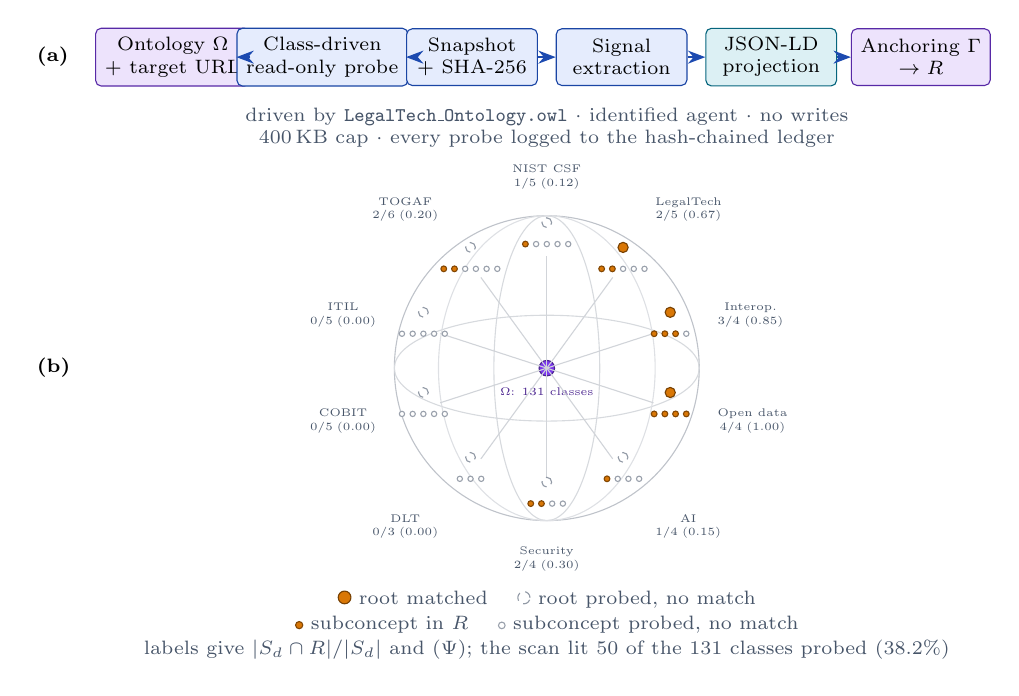
\begin{tikzpicture}[scale=1, transform shape,
  stg/.style={draw=lsBlue!70!black, rounded corners=2pt, minimum width=1.66cm, minimum height=0.72cm, align=center, font=\scriptsize, fill=lsBlue!12},
  arr/.style={-{Stealth[length=2.2mm]}, thick, lsBlue!75!black},
  rlit/.style={circle, fill=lsAmber, draw=lsAmber!55!black, inner sep=0pt, minimum size=4.6pt},
  rdim/.style={circle, fill=white, draw=lsSlate!60, densely dashed, inner sep=0pt, minimum size=4.4pt},
  slit/.style={circle, fill=lsAmber, draw=lsAmber!60!black, inner sep=0pt, minimum size=2.6pt},
  sdim/.style={circle, fill=white, draw=lsSlate!55, inner sep=0pt, minimum size=2.4pt},
  cst/.style={font=\tiny, text=lsSlate, align=center}]
\node[stg, draw=lsViolet!70!black, fill=lsViolet!14] (s0) at (0,0) {Ontology $\Omega$\\\scriptsize + target URL};
\node[stg] (s1) at (1.90,0) {Class-driven\\read-only probe};
\node[stg] (s2) at (3.80,0) {Snapshot\\+ SHA-256};
\node[stg] (s3) at (5.70,0) {Signal\\extraction};
\node[stg, draw=lsCyan!70!black, fill=lsCyan!14] (s4) at (7.60,0) {JSON-LD\\projection};
\node[stg, draw=lsViolet!70!black, fill=lsViolet!14] (s5) at (9.50,0) {Anchoring $\Gamma$\\$\rightarrow R$};
\foreach \a/\b in {s0/s1,s1/s2,s2/s3,s3/s4,s4/s5}{\draw[arr] (\a) -- (\b);}
\node[font=\scriptsize, text=lsSlate, anchor=north, align=center] at (4.75,-0.52)
  {driven by \texttt{LegalTech\_Ontology.owl} $\cdot$ identified agent $\cdot$ no writes\\
   400\,KB cap $\cdot$ every probe logged to the hash-chained ledger};
\node[font=\scriptsize\bfseries, anchor=west] at (-1.85,0) {(\textbf{a})};

% ── (b) Esfera celeste: la ontología conduce el barrido y registra los aciertos ──
% REV2b: se restaura el panel y se completa con conteos |S_d∩R|/|S_d| por
% constelación, de modo que la figura transmita cómo se levanta la sombra
% a partir de la ontología y no sólo el estado final (Tabla 3).
\begin{scope}[shift={(4.75,-3.95)}, scale=0.80]
\draw[lsSlate!35] (0,0) circle (2.42);
\draw[lsSlate!22] (0,0) ellipse (2.42 and 0.84);
\draw[lsSlate!22] (0,0) ellipse (0.84 and 2.42);
\draw[lsSlate!18] (0,0) ellipse (1.72 and 2.42);
\node[circle, fill=lsViolet, draw=lsViolet!60!black, inner sep=0pt, minimum size=7pt] at (0,0) {};
\node[font=\tiny, text=lsViolet!60!black, anchor=north] at (0,-0.18) {$\Omega$: 131 classes};
\foreach \a in {90,54,18,-18,-54,-90,-126,-162,162,126}{\draw[lsSlate!25] (0,0) -- (\a:1.78);}
\lsconst{-18}{rlit}{-1.5/slit,-0.5/slit,0.5/slit,1.5/slit}
\node[cst, anchor=west] at (-18:2.72) {Open data\\4/4\;(1.00)};
\lsconst{18}{rlit}{-1.5/slit,-0.5/slit,0.5/slit,1.5/sdim}
\node[cst, anchor=west] at (18:2.72) {Interop.\\3/4\;(0.85)};
\lsconst{54}{rlit}{-2/slit,-1/slit,0/sdim,1/sdim,2/sdim}
\node[cst, anchor=south west] at (54:2.72) {LegalTech\\2/5\;(0.67)};
\lsconst{90}{rdim}{-2/slit,-1/sdim,0/sdim,1/sdim,2/sdim}
\node[cst, anchor=south] at (90:2.72) {NIST CSF\\1/5\;(0.12)};
\lsconst{126}{rdim}{-2.5/slit,-1.5/slit,-0.5/sdim,0.5/sdim,1.5/sdim,2.5/sdim}
\node[cst, anchor=south east] at (126:2.72) {TOGAF\\2/6\;(0.20)};
\lsconst{162}{rdim}{-2/sdim,-1/sdim,0/sdim,1/sdim,2/sdim}
\node[cst, anchor=east] at (162:2.72) {ITIL\\0/5\;(0.00)};
\lsconst{-162}{rdim}{-2/sdim,-1/sdim,0/sdim,1/sdim,2/sdim}
\node[cst, anchor=east] at (-162:2.72) {COBIT\\0/5\;(0.00)};
\lsconst{-126}{rdim}{-1/sdim,0/sdim,1/sdim}
\node[cst, anchor=north east] at (-126:2.72) {DLT\\0/3\;(0.00)};
\lsconst{-90}{rdim}{-1.5/slit,-0.5/slit,0.5/sdim,1.5/sdim}
\node[cst, anchor=north] at (-90:2.72) {Security\\2/4\;(0.30)};
\lsconst{-54}{rdim}{-1.5/slit,-0.5/sdim,0.5/sdim,1.5/sdim}
\node[cst, anchor=north west] at (-54:2.72) {AI\\1/4\;(0.15)};
\end{scope}
\node[font=\scriptsize\bfseries, anchor=west] at (-1.85,-3.95) {(\textbf{b})};
\node[font=\scriptsize, text=lsSlate, anchor=north, align=center] at (4.75,-6.65)
  {\tikz\node[rlit]{};~root matched \quad \tikz\node[rdim]{};~root probed, no match\\[1pt]
   \tikz\node[slit]{};~subconcept in $R$ \quad \tikz\node[sdim]{};~subconcept probed, no match\\[1pt]
   labels give $|S_d\cap R|/|S_d|$ and $(\Psi)$; the scan lit 50 of the 131 classes probed (38.2\%)};
\end{tikzpicture}

\caption{The GET-SDS acquisition process, driven by the ontology at both ends. (\textbf{a}) Pipeline: $\Omega$ declares what is worth looking for, the probe fetches only that, and every step is written to the hash-chained ledger. (\textbf{b}) The same ontology as a celestial sphere: each dimension is a constellation whose large marker is its root $r_d$ and whose small markers are its subconcepts $S_d$. The field starts uniformly dim and the scan lights only what it matches, so the figure shows the shadow being raised rather than its final state alone. Open data closes completely; interoperability and LegalTech match at the root and in part of their detail; TOGAF, NIST~CSF, security and AI match only below the root---an incomplete practice; COBIT, ITIL and DLT stay dark---an absent one. Marker positions are schematic; the counts are exact.\label{fig:getsds}}
\end{figure}

Algorithm~\ref{alg:sds} states the procedure executed on every run, so that a third party can re-run it at a new cut-off date and compare artefacts.

\begin{figure}[H]
\centering
\begin{minipage}{\textwidth}
\footnotesize
\refstepcounter{algo}\label{alg:sds}%
\rule{\textwidth}{0.6pt}\\[2pt]
\textbf{Algorithm \thealgo:} Digital shadow generation and semantic validation\\[-6pt]
\rule{\textwidth}{0.4pt}
\begin{tabbing}
xxx\=xx\=\kill
\textbf{Input:} seed targets $T$; ontology $\Omega$; dimensions $D$; weights $(w_r,w_s)$\\
\textbf{Output:} shadow $\Delta$; coverage set $R$; per-dimension $\Psi,\mathrm{sds},\delta$; index $L$\\[2pt]
1.\> derive the probe set $P$ from $\Omega$: each class $c\in C$ contributes its observable evidence pattern\\
2.\> \textbf{for each} $\tau\in T$, \textbf{for each} $\rho\in P$: fetch read-only (identified agent, 400\,KB cap);\\
\> store snapshot; log the probing class, URL, UTC timestamp, bytes, latency, SHA-256 and match outcome\\
3.\> verify integrity: re-hash each snapshot, abort on mismatch, append the run to the ledger\\
4.\> extract deterministic signals from the markup (generator, legacy links, JSON-LD, API)\\
5.\> project signals into $\Delta=G(V,E,\lambda)$ and serialise as JSON-LD with the \texttt{@context} of $\Omega$\\
6.\> \textbf{for each} $v\in V$: resolve $\Gamma(v)\subseteq C$ via \texttt{maltg:mapsTo}; reject dangling identifiers\\
7.\> $R \leftarrow \bigcup_{v\in V}\Gamma(v)$\hfill\textit{// Eq.~\eqref{eq:coverage-set}}\\
8.\> \textbf{for each} $d\in D$: $\Psi(d)\leftarrow$ Eq.~\eqref{eq:psi}; then $\mathrm{sds}(d)$ and $\delta(d)$ by Eq.~\eqref{eq:delta}\\
9.\> aggregate to $\Psi_{\mathrm{global}}$ (Eq.~\eqref{eq:global}); $L\leftarrow$ band; sort $D$ by $\delta$ descending\\
10.\> persist the dated artefact with the ontology and shadow digests
\end{tabbing}
\vspace{-6pt}\rule{\textwidth}{0.6pt}
\end{minipage}
\end{figure}

%% ============================================================
\section{Case Study and Results}
\label{sec:results}

The study applies LegalShadow to the public digital ecosystem of the Ecuadorian Judiciary Council (\texttt{funcionjudicial\-.gob\-.ec}) and validates the resulting shadow against the full ontology (131 classes, 144 relations, 14 cross-cutting), contrasted with a synthetic \emph{positive control}: a 39-component shadow authored to saturate the engine, whose role is to establish that the metric can approach unity on a well-anchored artefact.

\textbf{Scoring protocol.} The ontological scores $\sigma$ were not elicited ad hoc. Each of the ten dimensions has a versioned rubric fixing five observable levels (0, 25, 50, 75, 100) with explicit criteria---for TOGAF, for instance, level~50 requires the BDAT domains to be identified with named owners, and level~75 requires an operating ADM cycle with an architecture repository. A score with no associated evidence is flagged \emph{declared} rather than \emph{observed}, which is precisely what separates the declarative index of the next paragraph from the coverage figure that follows it. The rubric, the seed sources and the evidence manifests are versioned alongside the shadows, so the coding is auditable; it was, however, applied by the authors rather than by an independent panel (Section~\ref{sec:conclusions}).
% REV2 (3.2): se explicita qué parte del modelo depende de juicio experto y
% qué parte no, y cómo un tercero puede rehacer cada una por separado.
The model's two quantities differ in epistemic status, and separating them is what makes partial replication possible. $\mathrm{onto}(d)$ is expert-elicited, so a reviewer who disagrees with a level definition obtains different absolute $\delta$. $\Psi(d)$ is not: it is a deterministic function of the rule table and the stored snapshots, reproducible bit for bit and independent of the rubric. A third party who accepts the rubric can verify everything by rerunning the pipeline; one who rejects it can still recompute every $\Psi(d)$ from the published artefacts, substitute their own $\mathrm{onto}$ vector and derive their own agenda. That ordering is robust: since $\delta$ is monotone in $\mathrm{onto}$ at fixed $\Psi$, the seven dimensions with $\Psi<0.35$ hold the top seven positions under any assignment keeping AI, ITIL and security above 70.

% REV1 (H-8): las tres cardinalidades se definen para que no se confundan.
\textbf{Evidence corpus.} Over 17 dated runs between 2 July and 4 August 2026 the acquisition tier issued 187 read-only requests, of which 170 succeeded (90.9\%). Re-hashing every stored snapshot against its manifest yields \textbf{170 matches and 0 mismatches}: full integrity of the evidence base. The ledger holds 37 chained entries from \texttt{GENESIS} to head \texttt{6c7d2847932a606f}. % REV3: condensado.
Three cardinalities appear here and measure different things: a \emph{run} is one pass of the protocol; a \emph{shadow regeneration} is a run that also rebuilt $\Delta$ end to end, of which there are five; a \emph{ledger entry} records a run, a verification or a methodological decision, hence their larger number. Latencies (median 788.5~ms, p95 954.4~ms, range 67--2810~ms) confirm the probe imposes negligible load, a design requirement of the ethical protocol \cite{Krotov2020}.

% REV1 (H-9): se reporta la estabilidad de Psi, no sólo la del índice declarativo.
\textbf{Institutional shadow and declarative maturity.} The shadow from the 4 August run contains \textbf{34 components, 32 flows and 7 architectural layers} anchored to 11 seed sources, with anchoring \emph{total and referentially closed}: every component carries at least one anchor (mean 2.00, max 4) and all 50 distinct references resolve, with zero dangling identifiers. Signals show a modern portal on a generic content manager still surfacing 16 legacy links (6 JSF, 10 PHP), a confirmed case-consultation SPA with no documented public API, and the total absence of embedded JSON-LD despite declarative references to open data policies---exactly the gap between nominal publication and effective reuse reported in the open government literature \cite{Janssen2012,Attard2015}. The assessment over the four dimensions for which the institution publishes declarative evidence gives a global index of \textbf{46/100}, which $L$ places at Level 3 (``Defined''): data and semantic interoperability 28, integration architecture 42, declared transformation 55, regulatory compliance 58. Both this index and the coverage figures reported below were invariant across the five regenerated shadows: the only signal that drifted in the series was the legacy PHP count (13~$\rightarrow$~10 between 5 and 30 July), attributable to content editing on the observed portal, and that signal anchors no ontology class, so the coverage set $R$---and with it $\Psi_{\mathrm{global}}$---did not change.

% REV1 (H-7): 90.4 % y 7.1 recalculados sobre valores sin redondear.
% REV1 (H-10): alcance del control explicitado.
\textbf{Ten-dimension semantic validation.} Applying the engine of Section~\ref{sec:formal} to the same real shadow (Table~\ref{tab:validation}, Figure~\ref{fig:gaps}) gives $\Psi_{\mathrm{global}}=25.8/73.9=\mathbf{0.349}$: the shadow materialises only 34.9\% of the maturity the ontology prescribes, leaving an aggregate gap of 48.2 points (65.1\%). The positive control reaches $\Psi_{\mathrm{global}}=66.9/73.9=90.4\%$ with a residual gap of 7.1. This rules out a ceiling artefact in the scoring engine and shows that the low real coverage is a property of the observed ecosystem rather than of the instrument; it does not, on its own, establish construct validity, since the control was authored by the same team (Section~\ref{sec:conclusions}).

A result visible only through the shared apparatus is that both shadows light almost the same number of stars---50 of 131 for the real shadow against 51 for the control---yet their global coverage differs by a factor of 2.6. Coverage \emph{breadth} is not what $\Psi$ measures: \emph{which} concepts are anchored matters far more than how many. The control spreads its 51 anchors across all ten dimensions; the real ecosystem concentrates its 50 in open data, interoperability and LegalTech, leaving whole dimensions untouched. A naive count of evidenced nodes would have rated the two artefacts equivalent.

Figure~\ref{fig:gaps} renders the same table as three series ordered by decreasing $\delta$---light bars for what the ontology prescribes, dark for what the shadow delivers, dashed line for the difference---so that reading left to right gives the agenda directly. The shape carries the argument: the bar series converge only at the right-hand end, where open data and interoperability sit, and diverge almost completely on the left, where the enterprise frameworks are.

Three dimensions have \emph{zero} coverage because neither root nor subconcepts appear in $R$: service management (ITIL, $\delta=79.5$), control (COBIT, $\delta=62.7$) and distributed ledger ($\delta=52.4$). Four more are lit only below the root---AI, NIST CSF, security posture and TOGAF---which is a different condition and calls for different remediation. The single largest gap is AI integration ($\delta=82.4$), where a high ontological score (96.9) is almost entirely unrealised. Conversely open data attains full coverage and interoperability 0.85, reflecting genuine participation in the national open data catalogue.

% REV2 (3.4): el contraste 4 vs. 10 dimensiones se eleva a párrafo destacado.
\textbf{The two headline figures do not measure the same thing---and that is the finding.} It is tempting to read 46/100 against 34.9\% as a single quantity assessed twice, and that reading would be wrong. The 46/100 aggregates the \emph{four} dimensions on which the institution itself publishes declarative evidence: data and semantic interoperability, integration architecture, declared transformation, regulatory compliance. $\Psi_{\mathrm{global}}$ spans the \emph{ten} dimensions the ontology prescribes. Neither the scales nor the dimension sets coincide, so the comparison is not a difference of degree but a difference of frame: what an institution reports \emph{on its own terms} versus what its digital surface exposes \emph{on the frameworks' terms}. Read that way the result is sharper rather than weaker. An institution can only report progress on the dimensions it has chosen to instrument; the six dimensions missing from its own assessment---ITIL, COBIT, distributed ledger, AI, NIST CSF and security posture---are, without exception, the ones in which the ontology finds little or no machine-processable trace. The self-assessment is not merely optimistic in value; it is silent exactly where the deficit is.

\begin{table}[H]
\small
% REV1 (H-6, H-7): fila global re-rotulada y nota de agregación añadida.
\caption{Hierarchical coverage validation of the real institutional shadow, $(w_r,w_s)=(0.40,\,0.60)$. The last column reports the synthetic positive control for the same dimension. Aggregates follow Equation~\eqref{eq:global} with equal $\omega_d$ and are computed on unrounded values; $\Psi_{\mathrm{global}}$ is thus an $\mathrm{onto}$-weighted mean of the $\Psi(d)$ column, whose unweighted mean is 0.329 (real) and 0.900 (control).\label{tab:validation}}
\begin{tabularx}{\textwidth}{Xcccccc}
\toprule
\textbf{Dimension} & $\mathbf{onto(d)}$ & \textbf{Root} & $\mathbf{\Psi(d)}$ & $\mathbf{sds(d)}$ & $\boldsymbol{\delta}\mathbf{(d)}$ & $\mathbf{\Psi}$ \textbf{ctrl}\\
\midrule
AI integration            & 96.9 & No  & 0.150 & 14.5 & \textbf{82.4} & 0.85\\
Service management (ITIL) & 79.5 & No  & 0.000 & 0.0  & \textbf{79.5} & 1.00\\
Resilience (NIST CSF)     & 72.0 & No  & 0.120 & 8.6  & 63.4 & 1.00\\
Control (COBIT)           & 62.7 & No  & 0.000 & 0.0  & 62.7 & 1.00\\
Security posture          & 80.4 & No  & 0.300 & 24.1 & 56.3 & 1.00\\
Distributed ledger        & 52.4 & No  & 0.000 & 0.0  & 52.4 & 0.85\\
Governance (TOGAF)        & 60.3 & No  & 0.200 & 12.1 & 48.2 & 0.70\\
LegalTech domain          & 75.5 & Yes & 0.673 & 50.8 & 24.7 & 0.60\\
Interoperability          & 81.2 & Yes & 0.850 & 69.0 & 12.2 & 1.00\\
Open data                 & 78.5 & Yes & 1.000 & 78.5 & 0.0  & 1.00\\
\midrule
\textbf{Global (Eq.~\eqref{eq:global}, $\mathrm{onto}$-weighted)} & \textbf{73.9} & 3/10 & \textbf{0.349} & \textbf{25.8} & \textbf{48.2} & \textbf{0.904}\\
\bottomrule
\end{tabularx}
\end{table}

\begin{figure}[H]
\centering
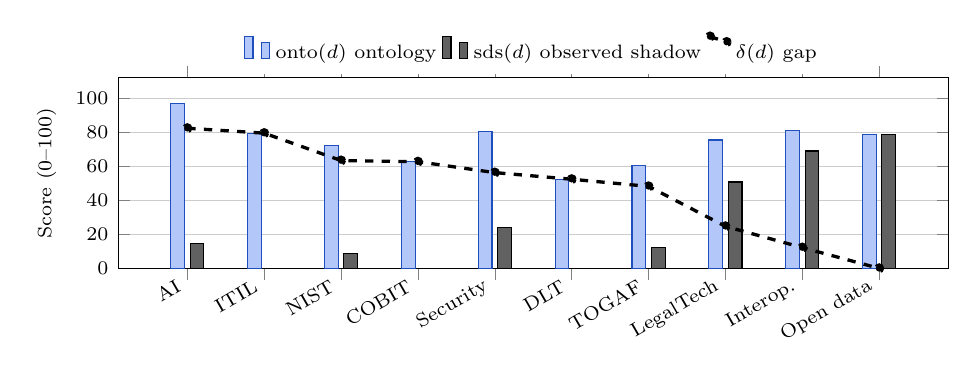
\begin{tikzpicture}
\begin{axis}[
  ybar,
  width=\textwidth, height=4.0cm,
  bar width=5pt,
  ymin=0, ymax=112,
  ylabel={Score (0--100)},
  ylabel style={font=\scriptsize},
  symbolic x coords={AI,ITIL,NIST,COBIT,Security,DLT,TOGAF,LegalTech,Interop.,Open data},
  xtick=data,
  x tick label style={rotate=30, anchor=east, font=\scriptsize},
  ytick={0,20,40,60,80,100},
  yticklabel style={font=\scriptsize},
  legend style={font=\scriptsize, at={(0.5,1.02)}, anchor=south, legend columns=3, draw=none},
  ymajorgrids, major grid style={black!20},
]
\addplot+[draw=lsBlue!80!black, fill=lsBlue!35] coordinates
  {(AI,96.9) (ITIL,79.5) (NIST,72.0) (COBIT,62.7) (Security,80.4) (DLT,52.4) (TOGAF,60.3) (LegalTech,75.5) (Interop.,81.2) (Open data,78.5)};
\addplot+[draw=black, fill=black!62] coordinates
  {(AI,14.5) (ITIL,0) (NIST,8.6) (COBIT,0) (Security,24.1) (DLT,0) (TOGAF,12.1) (LegalTech,50.8) (Interop.,69.0) (Open data,78.5)};
\addplot[sharp plot, very thick, dashed, black, mark=*, mark size=1.2pt] coordinates
  {(AI,82.4) (ITIL,79.5) (NIST,63.4) (COBIT,62.7) (Security,56.3) (DLT,52.4) (TOGAF,48.2) (LegalTech,24.7) (Interop.,12.2) (Open data,0)};
\legend{$\mathrm{onto}(d)$ ontology, $\mathrm{sds}(d)$ observed shadow, $\delta(d)$ gap}
\end{axis}
\end{tikzpicture}
\caption{Ontological versus effective maturity of the real institutional shadow, ordered by decreasing gap. The dashed line traces $\delta(d)$ and constitutes the remediation agenda.\label{fig:gaps}}
\end{figure}

%% ============================================================
\section{Discussion and Conclusions}
\label{sec:conclusions}

\textbf{Declarative maturity is not machine-actionable governance.} On the four dimensions it instruments itself, the institution scores 46/100, a figure a conventional assessment would report as reasonable progress. Evaluated against the semantics of the ten dimensions prescribed by the very frameworks it invokes, its observable ecosystem materialises 34.9\%, with three dimensions at zero anchored concepts and four more lit only below the root. The instrument separates what an institution \emph{declares} from what its digital surface \emph{exposes in machine-processable form}---quantities that maturity questionnaires conflate, and that differ not only in value but in the set of dimensions they can address at all.

% REV2 (3.5): el hallazgo reflexivo se desarrolla en sus dos consecuencias,
% una metodológica (piso de medición) y otra prescriptiva (agenda concreta).
\textbf{A reflexive finding, and its two consequences.} The most deficient signal is precisely the absence of embedded JSON-LD and of a documented public API: the observed institution lacks the very instrument---structured data---that the digital shadow uses to represent it. This is not only an ironic observation; it has a methodological and a prescriptive consequence, and the two pull in opposite directions.

The methodological consequence is a \emph{measurement floor}. Any instrument of this family resolves governance only to the granularity at which the observed institution has chosen to structure its public surface: where a portal publishes prose, the shadow records that a page exists but cannot anchor what it asserts. Coverage is therefore a joint property of the ecosystem and of its publication practices, and $\Psi$ conflates them---a low score cannot distinguish an institution that does not govern from one that governs without publishing structured evidence of it. No refinement of $\Gamma$ removes this bound; only the institution can, by publishing. The corollary matters for longitudinal use: adopting semantic markup would raise measured coverage with no change in underlying governance, an effect repeated measurement must control for.

The prescriptive consequence is that the highest-leverage remediation is also the cheapest. Three publication acts move several dimensions at once: embedding \texttt{schema.org} JSON-LD, which improves findability \cite{Guha2016} and anchors open data and interoperability; documenting the case-consultation API that demonstrably already exists behind the single-page application, converting an opaque service into an auditable one; and publishing a machine-readable governance manifest declaring frameworks in use, owners and review cycles---the minimum artefact that would let any external observer anchor the roots of ITIL, COBIT and security posture that are currently unreachable. None requires reforming how the institution is governed; all three change what can be known about it from outside, and let third parties build value-added services on judicial data \cite{Attard2015,Wilkinson2016}.

\textbf{Contribution to an open problem.} Karabulut et al.\ note the absence of methods to verify that a twin materialises its semantic model \cite{Karabulut2024}. $\Psi$ offers an operational answer: bounded, monotone, computable in linear time and interpretable dimension by dimension, it enables continuous audits of ontology--artefact alignment, while its root/subconcept decomposition localises the deficit---separating ITIL (absent) from TOGAF (incomplete) and interoperability (near-complete), distinctions no scalar score expresses. % REV3: condensado

% REV1 (H-10): se añade la limitación de validez de constructo del control.
\textbf{Limitations.} The shadow observes only the \emph{public surface}: scores are \emph{observable} maturity, a lower bound on real maturity, and dimensions such as ITIL or COBIT may operate internally without public trace, so their zero coverage measures published evidence rather than practice. The ontological scores $\sigma$ were assigned by the authors against the versioned rubric rather than elicited from an independent panel; no Delphi round, content-validity ratio \cite{Lawshe1975} or inter-rater agreement has yet been computed, so $\mathrm{onto}(d)$---and therefore the absolute value of $\delta$---carries unquantified judgement. The synthetic control is a positive control only: authored by the same team to saturate the engine, it bounds instrument artefacts but does not establish construct validity, which would require an artefact whose true coverage is known independently. The sensitivity sweep bounds the effect of $(w_r,w_s)$ but not that of $\sigma$. Aggregation uses equal dimension weights. External validity is limited to one institution studied in depth over one month, so the reported stability of $\Psi_{\mathrm{global}}$ speaks to instrument repeatability, not to the ecosystem's behaviour over longer horizons. Signal detection depends on portal markup stability; the cryptographic record attenuates, without eliminating, observer drift.

% REV2 (3.1): límites de generalización y protocolo concreto de transferencia.
\textbf{External validity and how to transfer the method.} The empirical claim is deliberately narrow---one institution, one month, its public surface---and three generalisations must not be read into it. The \emph{numerical} result generalises to nothing: 46/100 and $\Psi_{\mathrm{global}}=34.9\%$ describe the Ecuadorian Judiciary Council in August 2026. The \emph{diagnostic pattern}---high declarative maturity alongside low semantic coverage concentrated in open data---is a hypothesis the single case makes plausible and only a multi-institutional study can test; the publication-versus-reuse gap reported across hundreds of portals \cite{Janssen2012,Attard2015,Neumaier2016} suggests it is not idiosyncratic, but that is inference by analogy. Only the \emph{instrument} generalises. Transfer takes four steps, of which only the second costs anything. (1)~Replace the seed file: the target is already a parameter. (2)~Localise the rule table of $\Gamma$: roughly a fifth of the rules key on national artefacts---the Ecuadorian catalogue, national interoperability schemes---and must be re-expressed against equivalent infrastructure, the one step demanding domain knowledge and the real obstacle to naive reuse. (3)~Leave $\Omega$ and its rubric unchanged where the frameworks are international, which covers eight of ten dimensions. (4)~Compare only $\Psi$ and $\delta$ across institutions, never raw signal counts, since portal technologies differ. Comparability rests on holding the ontology fixed while the rule table varies---the discipline that makes urban twins comparable across cities \cite{Shahat2021,Haraguchi2024}---and whether it survives contact with a second jurisdiction is untested.

% REV1 (m-10): se suaviza el claim de neutralidad geográfica, no demostrado.
\textbf{Conclusions and future work.} LegalShadow instantiates the digital shadow paradigm over a judicial technological ecosystem with three distinctive properties: automatic generation from public web evidence with cryptographically verifiable provenance, semantic grounding in a multi-standard governance ontology serialised in JSON-LD, and quantitative validation through $\Psi$ and $\delta$. Every figure reported here is recomputable by a third party from the published rubric and the dated artefacts, which is the property that turns the instrument into an audit rather than an assessment. The ontology encodes international frameworks, the protocol runs over standard HTTP and the context reuses global vocabularies, so the parts that would normally block reuse are not country-specific; what is country-specific is the rule table of $\Gamma$, and the transfer protocol above states exactly which fifth of it must be rewritten. Dated shadows per institution would then enable longitudinal and cross-sectional comparison, extending to justice the logic of comparable urban twins \cite{Shahat2021,Haraguchi2024}. Future work targets multi-institutional studies with full $\Psi/\delta$ evaluation per institution, independent elicitation of $\sigma$ to remove the judgement now embedded in $\mathrm{onto}(d)$, assisted loop closure preserving human decision under MAPE-K \cite{Kephart2003}, automatic ontology alignment to enrich $\Gamma$ \cite{Hogan2021}, and a behavioural dimension built on procedural performance indicators \cite{Medvedeva2020}.

\authorcontributions{
    Conceptualisation, methodology, software, 
    investigation, data curation and
    writing---original draft preparation,               P.M.P.-A.;
    validation and formal analysis,                     P.M.P.-A. and E.J.S.-C.;
    writing---review and editing, and visualisation,    P.M.P.-A., E.J.S.-C. and V.V.V.-B.;
    supervision and project administration,             E.J.S.-C.
    All authors have read and agreed to the published version of the manuscript.
}

\funding{This research received no external funding.}
\dataavailability{
% REV3: depósito único de este artefacto (LegalShadow, Zenodo v1.0).
    All artefacts of this study---the LegalShadow source code, the OWL governance ontology, the versioned scoring rubric that fixes $\mathrm{onto}(d)$, the \emph{signal}$\rightarrow$\emph{class} rule table that constitutes $\Gamma$, the dated JSON-LD shadows and the SHA-256 evidence manifests---are openly available without restriction at Zenodo (DOI:~10.5281/zenodo.21942315) \cite{paccha2026zenodo} and at \texttt{https://github.com/patmic/ArchLab}. Publishing the rubric and the rule table alongside the snapshots is what makes the two-level replication described in Section~\ref{sec:results} possible: $\Psi$ can be recomputed without rerunning acquisition, and $\mathrm{onto}$ can be replaced by a reviewer's own values. The evidence base reported here corresponds to ledger head \texttt{6c7d2847932a606f}, which any third party can recompute from the published manifests. Observed data originate exclusively from public resources of the Ecuadorian Judiciary Council.
    \\
    \textbf{The code and instructions to reproduce the setup are available at:}
    \begin{itemize}
        \item git clone https://github.com/patmic/ArchLab,
        \item docker compose up -d -{}-build
        \item and, access the dashboard at http://localhost:8080.
    \end{itemize}
}
\institutionalreview{Not applicable.}
\informedconsent{Not applicable.}
\acknowledgments{The authors acknowledge the open-source ontology engineering ecosystem
(\texttt{rdflib}, \texttt{pyvis}, OWLready2).}
\conflictsofinterest{The authors declare no conflicts of interest.}

\begin{adjustwidth}{-\extralength}{0cm}
\reftitle{References}
\bibliography{ICI2ST_LegalShadow_Ref}
\end{adjustwidth}

\PublishersNote{}
\end{document}
